
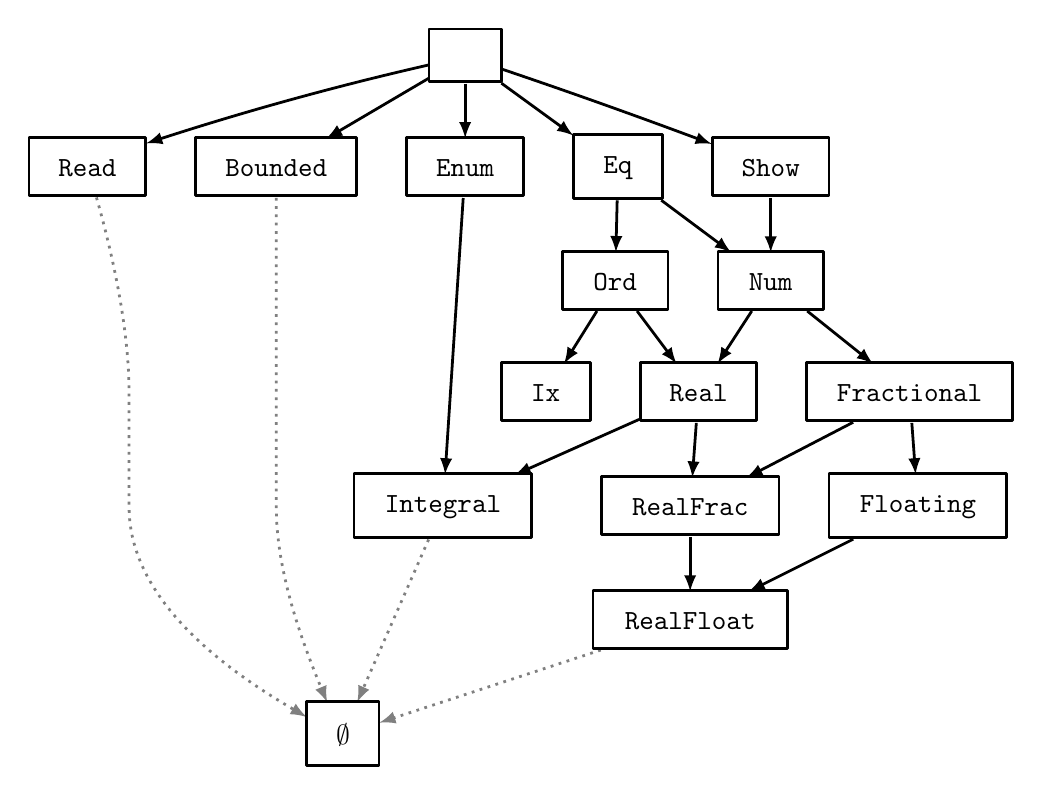
\begin{tikzpicture}[>=latex,line join=bevel,]
  \pgfsetlinewidth{1bp}
%%
\pgfsetcolor{black}
  % Edge: \texttt{Eq} -> \texttt{Num}
  \draw [->] (227.61bp,204.36bp) .. controls (232.91bp,200.42bp) and (238.92bp,195.93bp)  .. (252.67bp,185.69bp);
  % Edge: \texttt{Show} -> \texttt{Num}
  \draw [->] (267bp,205.23bp) .. controls (267bp,202.29bp) and (267bp,199bp)  .. (267bp,185.56bp);
  % Edge: \kindStar -> \texttt{Enum}
  \draw [->] (157bp,246.32bp) .. controls (157bp,243.45bp) and (157bp,240.19bp)  .. (157bp,226.72bp);
  % Edge: \kindStar -> \texttt{Read}
  \draw [->] (143.79bp,253.06bp) .. controls (125.17bp,248.8bp) and (89.974bp,240.34bp)  .. (42.187bp,224.85bp);
  % Edge: \kindStar -> \texttt{Show}
  \draw [->] (170.09bp,251.62bp) .. controls (184.37bp,246.79bp) and (208.09bp,238.66bp)  .. (245.74bp,224.64bp);
  % Edge: \texttt{Floating} -> \texttt{RealFloat}
  \draw [->] (296.72bp,82.361bp) .. controls (287.84bp,77.922bp) and (277.59bp,72.796bp)  .. (259.09bp,63.547bp);
  % Edge: \texttt{RealFloat} -> \emptyset
  \pgfsetcolor{gray}
  \draw [->,dotted] (205.81bp,42.441bp) .. controls (183.86bp,35.241bp) and (155.32bp,25.882bp)  .. (126.11bp,16.3bp);
  % Edge: \texttt{Fractional} -> \texttt{Floating}
  \pgfsetcolor{black}
  \draw [->] (317.79bp,124.23bp) .. controls (317.98bp,121.65bp) and (318.19bp,118.8bp)  .. (319.14bp,105.71bp);
  % Edge: \texttt{Num} -> \texttt{Fractional}
  \draw [->] (280.14bp,164.49bp) .. controls (284.92bp,160.66bp) and (290.46bp,156.23bp)  .. (303.78bp,145.58bp);
  % Edge: \kindStar -> \texttt{Eq}
  \draw [->] (170.03bp,246.52bp) .. controls (175.36bp,242.65bp) and (181.7bp,238.03bp)  .. (195.91bp,227.7bp);
  % Edge: \texttt{Real} -> \texttt{Integral}
  \draw [->] (219.66bp,125.49bp) .. controls (209.11bp,120.79bp) and (196.09bp,114.99bp)  .. (174.81bp,105.5bp);
  % Edge: \texttt{Real} -> \texttt{RealFrac}
  \draw [->] (240.21bp,124.23bp) .. controls (240bp,121.29bp) and (239.76bp,118bp)  .. (238.77bp,104.56bp);
  % Edge: \texttt{Enum} -> \texttt{Integral}
  \draw [->] (156.29bp,205.17bp) .. controls (154.98bp,185.17bp) and (152.15bp,142.07bp)  .. (149.77bp,105.69bp);
  % Edge: \texttt{Bounded} -> \emptyset
  \pgfsetcolor{gray}
  \draw [->,dotted] (89bp,205.26bp) .. controls (89bp,189.74bp) and (89bp,160.17bp)  .. (89bp,135bp) .. controls (89bp,135bp) and (89bp,135bp)  .. (89bp,94bp) .. controls (89bp,72.706bp) and (96.547bp,49.509bp)  .. (107.31bp,23.637bp);
  % Edge: \texttt{Ord} -> \texttt{Ix}
  \pgfsetcolor{black}
  \draw [->] (204.43bp,164.49bp) .. controls (202.44bp,161.3bp) and (200.18bp,157.69bp)  .. (192.61bp,145.58bp);
  % Edge: \texttt{Eq} -> \texttt{Ord}
  \draw [->] (211.72bp,204.36bp) .. controls (211.65bp,201.7bp) and (211.58bp,198.79bp)  .. (211.26bp,185.69bp);
  % Edge: \texttt{Ord} -> \texttt{Real}
  \draw [->] (218.88bp,164.49bp) .. controls (221.34bp,161.21bp) and (224.14bp,157.48bp)  .. (233.07bp,145.58bp);
  % Edge: \texttt{Num} -> \texttt{Real}
  \draw [->] (260.17bp,164.49bp) .. controls (258.1bp,161.3bp) and (255.75bp,157.69bp)  .. (247.88bp,145.58bp);
  % Edge: \texttt{Fractional} -> \texttt{RealFrac}
  \draw [->] (296.66bp,124.44bp) .. controls (287.72bp,119.8bp) and (277.05bp,114.27bp)  .. (258.28bp,104.52bp);
  % Edge: \texttt{Read} -> \emptyset
  \pgfsetcolor{gray}
  \draw [->,dotted] (24.255bp,205.37bp) .. controls (28.666bp,190bp) and (36bp,160.6bp)  .. (36bp,135bp) .. controls (36bp,135bp) and (36bp,135bp)  .. (36bp,94bp) .. controls (36bp,61.56bp) and (68.42bp,36.694bp)  .. (99.938bp,18.326bp);
  % Edge: \texttt{Integral} -> \emptyset
  \draw [->,dotted] (143.84bp,82.251bp) .. controls (138.23bp,69.464bp) and (129.14bp,48.756bp)  .. (118.15bp,23.727bp);
  % Edge: \texttt{RealFrac} -> \texttt{RealFloat}
  \pgfsetcolor{black}
  \draw [->] (238bp,83.228bp) .. controls (238bp,80.286bp) and (238bp,76.996bp)  .. (238bp,63.559bp);
  % Edge: \kindStar -> \texttt{Bounded}
  \draw [->] (143.89bp,248.29bp) .. controls (135.93bp,243.61bp) and (125.49bp,237.46bp)  .. (106.96bp,226.56bp);
  % Node: \texttt{Real}
\begin{scope}
  \definecolor{strokecol}{rgb}{0.0,0.0,0.0};
  \pgfsetstrokecolor{strokecol}
  \draw (262bp,146bp) -- (220bp,146bp) -- (220bp,125bp) -- (262bp,125bp) -- cycle;
  \draw (241bp,135bp) node {$\texttt{Real}$};
\end{scope}
  % Node: \texttt{Show}
\begin{scope}
  \definecolor{strokecol}{rgb}{0.0,0.0,0.0};
  \pgfsetstrokecolor{strokecol}
  \draw (288bp,227bp) -- (246bp,227bp) -- (246bp,206bp) -- (288bp,206bp) -- cycle;
  \draw (267bp,216bp) node {$\texttt{Show}$};
\end{scope}
  % Node: \texttt{Ord}
\begin{scope}
  \definecolor{strokecol}{rgb}{0.0,0.0,0.0};
  \pgfsetstrokecolor{strokecol}
  \draw (230bp,186bp) -- (192bp,186bp) -- (192bp,165bp) -- (230bp,165bp) -- cycle;
  \draw (211bp,175bp) node {$\texttt{Ord}$};
\end{scope}
  % Node: \texttt{Enum}
\begin{scope}
  \definecolor{strokecol}{rgb}{0.0,0.0,0.0};
  \pgfsetstrokecolor{strokecol}
  \draw (178bp,227bp) -- (136bp,227bp) -- (136bp,206bp) -- (178bp,206bp) -- cycle;
  \draw (157bp,216bp) node {$\texttt{Enum}$};
\end{scope}
  % Node: \texttt{Ix}
\begin{scope}
  \definecolor{strokecol}{rgb}{0.0,0.0,0.0};
  \pgfsetstrokecolor{strokecol}
  \draw (202bp,146bp) -- (170bp,146bp) -- (170bp,125bp) -- (202bp,125bp) -- cycle;
  \draw (186bp,135bp) node {$\texttt{Ix}$};
\end{scope}
  % Node: \texttt{Integral}
\begin{scope}
  \definecolor{strokecol}{rgb}{0.0,0.0,0.0};
  \pgfsetstrokecolor{strokecol}
  \draw (181bp,106bp) -- (117bp,106bp) -- (117bp,83bp) -- (181bp,83bp) -- cycle;
  \draw (149bp,94bp) node {$\texttt{Integral}$};
\end{scope}
  % Node: \texttt{Bounded}
\begin{scope}
  \definecolor{strokecol}{rgb}{0.0,0.0,0.0};
  \pgfsetstrokecolor{strokecol}
  \draw (118bp,227bp) -- (60bp,227bp) -- (60bp,206bp) -- (118bp,206bp) -- cycle;
  \draw (89bp,216bp) node {$\texttt{Bounded}$};
\end{scope}
  % Node: \kindStar
\begin{scope}
  \definecolor{strokecol}{rgb}{0.0,0.0,0.0};
  \pgfsetstrokecolor{strokecol}
  \draw (170bp,266bp) -- (144bp,266bp) -- (144bp,247bp) -- (170bp,247bp) -- cycle;
  \draw (157bp,256bp) node {$\kindStar$};
\end{scope}
  % Node: \texttt{RealFrac}
\begin{scope}
  \definecolor{strokecol}{rgb}{0.0,0.0,0.0};
  \pgfsetstrokecolor{strokecol}
  \draw (270bp,105bp) -- (206bp,105bp) -- (206bp,84bp) -- (270bp,84bp) -- cycle;
  \draw (238bp,94bp) node {$\texttt{RealFrac}$};
\end{scope}
  % Node: \texttt{Fractional}
\begin{scope}
  \definecolor{strokecol}{rgb}{0.0,0.0,0.0};
  \pgfsetstrokecolor{strokecol}
  \draw (354bp,146bp) -- (280bp,146bp) -- (280bp,125bp) -- (354bp,125bp) -- cycle;
  \draw (317bp,135bp) node {$\texttt{Fractional}$};
\end{scope}
  % Node: \texttt{Floating}
\begin{scope}
  \definecolor{strokecol}{rgb}{0.0,0.0,0.0};
  \pgfsetstrokecolor{strokecol}
  \draw (352bp,106bp) -- (288bp,106bp) -- (288bp,83bp) -- (352bp,83bp) -- cycle;
  \draw (320bp,94bp) node {$\texttt{Floating}$};
\end{scope}
  % Node: \texttt{Eq}
\begin{scope}
  \definecolor{strokecol}{rgb}{0.0,0.0,0.0};
  \pgfsetstrokecolor{strokecol}
  \draw (228bp,228bp) -- (196bp,228bp) -- (196bp,205bp) -- (228bp,205bp) -- cycle;
  \draw (212bp,216bp) node {$\texttt{Eq}$};
\end{scope}
  % Node: \texttt{RealFloat}
\begin{scope}
  \definecolor{strokecol}{rgb}{0.0,0.0,0.0};
  \pgfsetstrokecolor{strokecol}
  \draw (273bp,64bp) -- (203bp,64bp) -- (203bp,43bp) -- (273bp,43bp) -- cycle;
  \draw (238bp,53bp) node {$\texttt{RealFloat}$};
\end{scope}
  % Node: \emptyset
\begin{scope}
  \definecolor{strokecol}{rgb}{0.0,0.0,0.0};
  \pgfsetstrokecolor{strokecol}
  \draw (126bp,24bp) -- (100bp,24bp) -- (100bp,1bp) -- (126bp,1bp) -- cycle;
  \draw (113bp,12bp) node {$\emptyset$};
\end{scope}
  % Node: \texttt{Num}
\begin{scope}
  \definecolor{strokecol}{rgb}{0.0,0.0,0.0};
  \pgfsetstrokecolor{strokecol}
  \draw (286bp,186bp) -- (248bp,186bp) -- (248bp,165bp) -- (286bp,165bp) -- cycle;
  \draw (267bp,175bp) node {$\texttt{Num}$};
\end{scope}
  % Node: \texttt{Read}
\begin{scope}
  \definecolor{strokecol}{rgb}{0.0,0.0,0.0};
  \pgfsetstrokecolor{strokecol}
  \draw (42bp,227bp) -- (0bp,227bp) -- (0bp,206bp) -- (42bp,206bp) -- cycle;
  \draw (21bp,216bp) node {$\texttt{Read}$};
\end{scope}
%
\end{tikzpicture}

